\subsection{Training results}
\label{subsec:train-res}

We have \emph{combined} the different components explained in Section~\ref{sec:methodology} and we conducted a thorough experimentation process to identify the best-performing system for our task. 
By tuning the parameters of each component and selecting the optimal ones, we were able to build a 
system that addresses the persistence issue of \ac{IR} systems.
In Table~\ref{tab:map-ndcg-table} are reported the \ac{MAP} and \ac{nDCG} scores obtained on those systems.

\begin{table}[tbp]
\caption{\ac{nDCG} and \ac{MAP} values on train collection}
  \label{tab:map-ndcg-table}
    \centering
    \begin{tabular}{|p{0.7\linewidth}|p{0.075\linewidth}|p{0.075\linewidth}|}
	\toprule
	\textbf{Run name} & \textbf{nDCG} & \textbf{MAP} \\
	\midrule
        \raggedright FADERIC\_French-BM25-Stop50-LightStem-Shingle-Fuzzy-SynCustom-Rerank20W6 & 0.4274 & 0.2671 \\ 
        FADERIC\_French-BM25-Stop50-LightStem-Shingle-Fuzzy-Rerank30 & 0.4230 & 0.2632 \\ 
        FADERIC\_French-BM25-Stop50-LightStem-Shingle-Fuzzy-SynCustom & 0.4079 & 0.2416 \\ 
        FADERIC\_French-BM25Tuned-Stop50-LightStem-Shingle-Fuzzy & 0.4047 & 0.2383 \\ 
        FADERIC\_French-BM25-StopDefault-SnowStem & 0.3786 & 0.2110 \\ 
        FADERIC\_English-BM25-Stop50-KStem-Shingle-Fuzzy-SynPOS\\-Rerank30 & 0.3271 & 0.1877 \\ 
        FADERIC\_English-BM25-Stop50-KStem-Shingle-Fuzzy-Rerank30 & 0.3527 & 0.1873 \\ 
        FADERIC\_French-BM25-Stop50-LightStem-Shingle-Fuzzy\\-TrainedRerank30 & 0.3599 & 0.1799 \\ 
        FADERIC\_French-LMDirichlet-Stop50-LightStem & 0.3398 & 0.1731 \\ 
        FADERIC\_English-BM25-Stop50-KStem-Shingle-Fuzzy-SynPOS & 0.3081 & 0.1634 \\ 
        FADERIC\_English-BM25-StopDefault-SnowStem & 0.2927 & 0.1490 \\ 
        FADERIC\_English-LMDirichlet-Stop50-KStem & 0.2612 & 0.1228 \\ 
	\bottomrule
    \end{tabular}
\end{table}

The keywords reported in the names of the runs have the following meanings:
\begin{itemize}
	\item French: used documents and queries from the French collection
	\item English: used documents and queries from the English collection
	\item BM25: used Okapi BM25 similarity (with default parameters)
	\item BM25Tuned: used Okapi BM25 similarity, with parameters tuned on training collection: k1=1.6 and b=0.7
	\item LMDirichlet: used Dirichlet smoothing (with default parameter)
	\item StopDefault: used Lucene's default stop words list
	\item Stop50: used stoplist built by picking the 50 most frequent terms in the documents indexed without stoplist and stemming
	\item LightStem: used the Light stemmer
	\item KStem: used Krovetz stemmer
	\item SnowStem: the Snowball stemmer
	\item Shingle: used word N-grams (max window size = 3) query expansion
	\item Fuzzy: used fuzzyness (threshold parameter = 10) query expansion
	\item SynCustom: used custom synonyms list
	\item SynPOS: used WordNet synonym list together with OpenNLP \ac{PoS} tagging
	\item Rererank20W6: used reranker, reranking 20 documents with weight 0.6 given to the reranker scores
	\item Rererank30: used reranker, reranking 30 documents with weight 1 given to the reranker scores
	\item TrainedRerank30: used reranker, reranking 30 documents using our custom model
\end{itemize}

During the tuning of our system, we primarily focused on \ac{MAP} and \ac{nDCG}. However, in order to perform a more \emph{comprehensive} analysis, 
we also considered additional measures such as Precision and Recall: the first one is the fraction of retrieved 
documents that are relevant to the user's query, indicating a measure of the accuracy of the system,
while with the second is a measure of the completeness of the system in retrieving all relevant results, 
computed by the fraction of relevant documents retrieved.

In Figure~\ref{fig:precision-recall-curve}, we show the \emph{interpolated} Precision-Recall curve, which can be useful to show the inverse relationship between Precision and Recall, indicating the \emph{trade-off} between these two measures.

\begin{figure}[tbp]
  \centering
  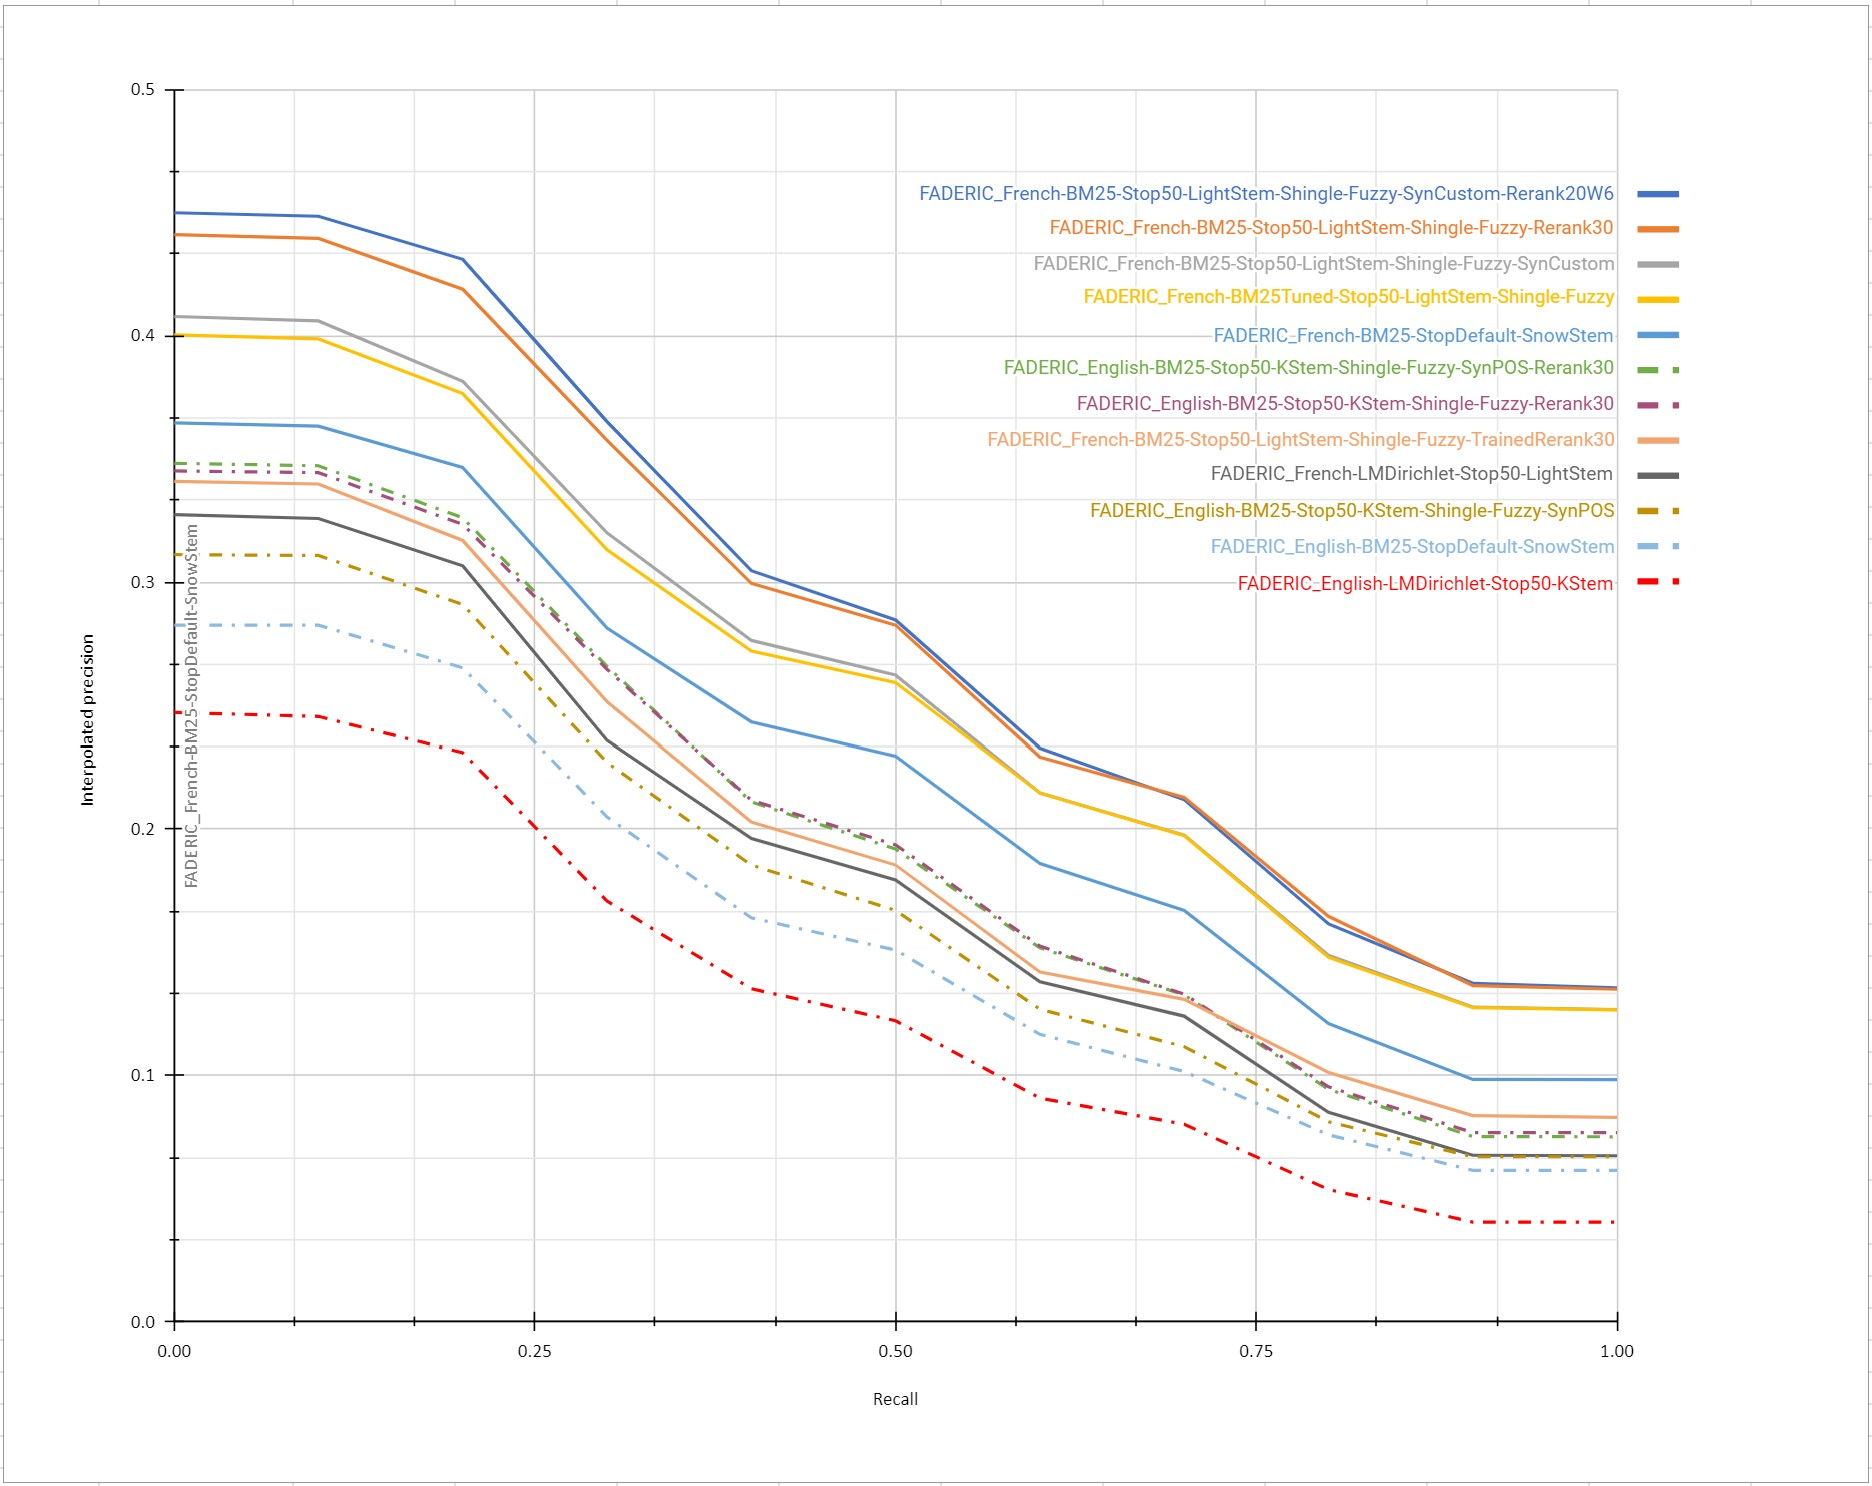
\includegraphics[width=1\linewidth]{figure/prec-recall.jpg}
  \caption{Interpolated Precision-Recall curve on train collection}
  \label{fig:precision-recall-curve}
\end{figure}

\pagebreak

In Table~\ref{tab:all-measures-french} and in Table~\ref{tab:all-measures-english} we have reported a more complete list of scores respectively for the French and English runs. For space reasons, we label the runs as: 

\begin{itemize}
	\item fr\_1 = FADERIC\_French-BM25-Stop50-LightStem-Shingle-Fuzzy-SynCustom\\-Rerank20W6
	\item fr\_2 = FADERIC\_French-BM25-Stop50-LightStem-Shingle-Fuzzy-Rerank30
	\item fr\_3 = FADERIC\_French-BM25-Stop50-LightStem-Shingle-Fuzzy-SynCustom
	\item fr\_4 = FADERIC\_French-BM25Tuned-Stop50-LightStem-Shingle-Fuzzy
	\item fr\_5 = FADERIC\_French-BM25-StopDefault-SnowStem
	\item fr\_6 = FADERIC\_French-BM25-Stop50-LightStem-Shingle-Fuzzy-TrainedRerank30
	\item fr\_7 = FADERIC\_French-LMDirichlet-Stop50-LightStem
	\item en\_1 = FADERIC\_English-BM25-Stop50-KStem-Shingle-Fuzzy-SynPOS-Rerank30
	\item en\_2 = FADERIC\_English-BM25-Stop50-KStem-Shingle-Fuzzy-Rerank30
	\item en\_3 = FADERIC\_English-BM25-Stop50-KStem-Shingle-Fuzzy-SynPOS
	\item en\_4 = FADERIC\_English-BM25-StopDefault-SnowStem
	\item en\_5 =FADERIC\_English-LMDirichlet-Stop50-KStem
\end{itemize}

\begin{table}[tbp]
\caption{Measures for French runs on train collection}
  \label{tab:all-measures-french}
    \centering
    \begin{tabular}{|l|l|l|l|l|l|l|l|l|l|}
    	\toprule
        runid & all & fr\_1 & fr\_2 & fr\_3 & fr\_4 & fr\_5 & fr\_6 & fr\_7  \\
	\midrule
        num\_q & all & 672 & 672 & 672 & 672 & 672 & 672 & 672  \\ 
        num\_ret & all & 660838 & 660838 & 660838 & 660838 & 658471 & 660838 & 658512  \\ 
        num\_rel & all & 2626 & 2626 & 2626 & 2626 & 2626 & 2626 & 2626  \\ 
        num\_rel\_ret & all & 2316 & 2318 & 2316 & 2323 & 2271 & 2318 & 2156  \\ \midrule
	ndcg & all & \textbf{0.4274} & 0.4230 & 0.4079 & 0.4047 & 0.3786 & 0.3599 & 0.3398  \\ \midrule
        map & all & \textbf{0.2670} & 0.2632 & 0.2416 & 0.2383 & 0.2110 & 0.1799 & 0.1731  \\ 
        gm\_map & all & \textbf{0.0786} & 0.0765 & 0.0702 & 0.0696 & 0.0545 & 0.0552 & 0.0394  \\ \midrule
        Rprec & all & \textbf{0.2280} & 0.2278 & 0.1987 & 0.1946 & 0.1747 & 0.1365 & 0.1469  \\ 
        bpref & all & \textbf{0.4128} & 0.4122 & 0.4085 & 0.4063 & 0.3753 & 0.3701 & 0.3561  \\ 
        recip\_rank & all & 0.4222 & 0.4140 & 0.3824 & 0.3734 & 0.3424 & 0.3170 & 0.3134  \\ \midrule
        iprec\_at\_recall\_0.00 & all & \textbf{0.4499} & 0.4410 & 0.4078 & 0.4003 & 0.3646 & 0.3409 & 0.3274  \\ 
        iprec\_at\_recall\_0.10 & all & \textbf{0.4485} & 0.4395 & 0.4060 & 0.3987 & 0.3633 & 0.3398 & 0.3258  \\ 
        iprec\_at\_recall\_0.20 & all & \textbf{0.4310} & 0.4189 & 0.3815 & 0.3765 & 0.3465 & 0.3169 & 0.3066  \\ 
        iprec\_at\_recall\_0.30 & all & \textbf{0.3651} & 0.3575 & 0.3200 & 0.3131 & 0.2813 & 0.2515 & 0.2359  \\ 
        iprec\_at\_recall\_0.40 & all & \textbf{0.3046} & 0.2995 & 0.2763 & 0.2720 & 0.2433 & 0.2030 & 0.1963  \\ 
        iprec\_at\_recall\_0.50 & all & \textbf{0.2846} & 0.2825 & 0.2623 & 0.2592 & 0.2296 & 0.1855 & 0.1795  \\ 
        iprec\_at\_recall\_0.60 & all & \textbf{0.2328} & 0.2293 & 0.2147 & 0.2147 & 0.1861 & 0.1421 & 0.1381  \\ 
        iprec\_at\_recall\_0.70 & all & 0.2120 & \textbf{0.2130} & 0.1976 & 0.1974 & 0.1671 & 0.1310 & 0.1242  \\ 
        iprec\_at\_recall\_0.80 & all & 0.1616 & \textbf{0.1647} & 0.1489 & 0.1481 & 0.1212 & 0.1013 & 0.0851  \\ 
        iprec\_at\_recall\_0.90 & all & \textbf{0.1375} & 0.1366 & 0.1279 & 0.1276 & 0.0985 & 0.0838 & 0.0677  \\ 
        iprec\_at\_recall\_1.00 & all & \textbf{0.1357} & 0.1351 & 0.1268 & 0.1267 & 0.0984 & 0.0831 & 0.0675  \\ \midrule
        P\_5 & all & \textbf{0.2074} & 0.2065 & 0.1875 & 0.1827 & 0.1637 & 0.1315 & 0.1375  \\ 
        P\_10 & all & \textbf{0.1603} & 0.1560 & 0.1472 & 0.1469 & 0.1332 & 0.1007 & 0.1088  \\ 
        P\_15 & all & 0.1233 & \textbf{0.1243} & 0.1183 & 0.1167 & 0.1090 & 0.0869 & 0.0889  \\ 
        P\_20 & all & 0.0990 & \textbf{0.1022} & 0.0990 & 0.0990 & 0.0901 & 0.0799 & 0.0753  \\ 
        P\_30 & all & \textbf{0.0748} & 0.0743 & \textbf{0.0748} & 0.0743 & 0.0683 & 0.0742 & 0.0580  \\ 
        P\_100 & all & 0.0279 & 0.0279 & 0.0279 & \textbf{0.0280} & 0.0267 & 0.0279 & 0.0232  \\ 
        P\_200 & all & 0.0150 & 0.0150 & 0.0150 & \textbf{0.0151} & 0.0146 & 0.0150 & 0.0133  \\ 
        P\_500 & all & \textbf{0.0065} & \textbf{0.0065} & \textbf{0.0065} & \textbf{0.0065} & 0.0064 & \textbf{0.0065} & 0.0060  \\ 
        P\_1000 & all & 0.0034 & 0.0034 & 0.0034 & \textbf{0.0035} & 0.0034 & 0.0034 & 0.0032  \\ \midrule
        recall\_5 & all & \textbf{0.2738} & 0.2732 & 0.2478 & 0.2417 & 0.2106 & 0.1749 & 0.1802  \\ 
        recall\_10 & all & \textbf{0.4167} & 0.4042 & 0.3830 & 0.3828 & 0.3402 & 0.2606 & 0.2789  \\ 
        recall\_15 & all & 0.4724 & \textbf{0.4757} & 0.4560 & 0.4499 & 0.4203 & 0.3366 & 0.3380  \\ 
        recall\_20 & all & 0.5034 & \textbf{0.5193} & 0.5032 & 0.5051 & 0.4595 & 0.4119 & 0.3814  \\ 
        recall\_30 & all & \textbf{0.5710} & 0.5657 & \textbf{0.5710} & 0.5677 & 0.5187 & 0.5651 & 0.4412  \\ 
        recall\_100 & all & 0.7022 & 0.7019 & 0.7022 & \textbf{0.7028} & 0.6688 & 0.7019 & 0.5816  \\ 
        recall\_200 & all & 0.7555 & 0.7560 & 0.7555 & \textbf{0.7587} & 0.7283 & 0.7560 & 0.6729  \\ 
        recall\_500 & all & 0.8219 & 0.8232 & 0.8219 & \textbf{0.8235} & 0.7994 & 0.8232 & 0.7574  \\ 
        recall\_1000 & all & 0.8663 & 0.8662 & 0.8663 & \textbf{0.8685} & 0.8485 & 0.8662 & 0.8072  \\
	\bottomrule
    \end{tabular}
\end{table}

\begin{table}[tbp]
\caption{Measures for English runs on train collection}
  \label{tab:all-measures-english}
    \centering
    \begin{tabular}{|l|l|l|l|l|l|l|}
    \toprule
	runid & all & en\_1 & en\_2 & en\_3 & en\_4 & en\_5  \\
	\midrule
        num\_q & all & 672 & 672 & 672 & 671 & 671  \\ 
        num\_ret & all & 655602 & 655602 & 655602 & 654919 & 654764  \\ 
        num\_rel & all & 2626 & 2626 & 2626 & 2623 & 2623  \\ 
        num\_rel\_ret & all & 1924 & 1915 & 1924 & 1878 & 1765  \\ \midrule
	ndcg & all & \textbf{0.3271} & 0.3257 & 0.3081 & 0.2927 & 0.2612  \\ \midrule
        map & all & \textbf{0.1877} & 0.1873 & 0.1634 & 0.1490 & 0.1228  \\ 
        gm\_map & all & \textbf{0.0221} & 0.0215 & 0.0195 & 0.0164 & 0.0122  \\ \midrule
        Rprec & all & 0.1706 & \textbf{0.1708} & 0.1385 & 0.1253 & 0.1092  \\ 
        bpref & all & \textbf{0.3536} & 0.3524 & 0.3417 & 0.3263 & 0.3139  \\ 
        recip\_rank & all & \textbf{0.3322} & 0.3289 & 0.2967 & 0.2697 & 0.2364  \\ \midrule
        iprec\_at\_recall\_0.00 & all & \textbf{0.3482} & 0.3451 & 0.3111 & 0.2825 & 0.2471  \\ 
        iprec\_at\_recall\_0.10 & all & \textbf{0.3472} & 0.3444 & 0.3108 & 0.2825 & 0.2455  \\ 
        iprec\_at\_recall\_0.20 & all & \textbf{0.3261} & 0.3234 & 0.2909 & 0.2652 & 0.2310  \\ 
        iprec\_at\_recall\_0.30 & all & \textbf{0.2658} & 0.2646 & 0.2270 & 0.2050 & 0.1709  \\ 
        iprec\_at\_recall\_0.40 & all & 0.2111 & \textbf{0.2118} & 0.1855 & 0.1641 & 0.1353  \\ 
        iprec\_at\_recall\_0.50 & all & 0.1920 & \textbf{0.1937} & 0.1671 & 0.1510 & 0.1223  \\ 
        iprec\_at\_recall\_0.60 & all & 0.1519 & \textbf{0.1526} & 0.1270 & 0.1168 & 0.0909  \\ 
        iprec\_at\_recall\_0.70 & all & 0.1328 & \textbf{0.1331} & 0.1118 & 0.1017 & 0.0803  \\ 
        iprec\_at\_recall\_0.80 & all & 0.0945 & \textbf{0.0955} & 0.0813 & 0.0760 & 0.0538  \\ 
        iprec\_at\_recall\_0.90 & all & 0.0753 & \textbf{0.0769} & 0.0671 & 0.0616 & 0.0406  \\ 
        iprec\_at\_recall\_1.00 & all & 0.0752 & \textbf{0.0769} & 0.0671 & 0.0616 & 0.0406  \\ \midrule
        P\_5 & all & \textbf{0.1542} & \textbf{0.1542} & 0.1345 & 0.1195 & 0.1019  \\ 
        P\_10 & all & \textbf{0.1137} & 0.1131 & 0.1042 & 0.0954 & 0.0793  \\ 
        P\_15 & all & \textbf{0.0904} & 0.0898 & 0.0835 & 0.0784 & 0.0650  \\ 
        P\_20 & all & \textbf{0.0745} & 0.0732 & 0.0705 & 0.0662 & 0.0543  \\ 
        P\_30 & all & 0.0536 & 0.053 & \textbf{0.0537} & 0.0513 & 0.0433  \\ 
        P\_100 & all & 0.0208 & \textbf{0.0209} & 0.0208 & 0.0201 & 0.0179  \\ 
        P\_200 & all & \textbf{0.0116} & 0.0115 & \textbf{0.0116} & 0.0113 & 0.0103  \\ 
        P\_500 & all &\textbf{ 0.0052} & \textbf{0.0052} & \textbf{0.0052} & 0.0051 & 0.0048  \\ 
        P\_1000 & all & \textbf{0.0029} & 0.0028 & \textbf{0.0029} & 0.0028 & 0.0026  \\ \midrule
        recall\_5 & all & \textbf{0.2020} & 0.2017 & 0.1710 & 0.1512 & 0.1329  \\ 
        recall\_10 & all & \textbf{0.2909} & 0.2887 & 0.2628 & 0.2437 & 0.1988  \\ 
        recall\_15 & all & \textbf{0.3430} & 0.3404 & 0.3155 & 0.2970 & 0.2432  \\ 
        recall\_20 & all & \textbf{0.3745} & 0.3683 & 0.3523 & 0.3318 & 0.2727  \\ 
        recall\_30 & all & 0.4010 & 0.3970 & \textbf{0.4018} & 0.3861 & 0.3281  \\ 
        recall\_100 & all & 0.5140 & \textbf{0.5167} & 0.5151 & 0.500 & 0.4486  \\ 
        recall\_200 & all & 0.5769 & 0.5754 & \textbf{0.5774} & 0.5630 & 0.5180  \\ 
        recall\_500 & all & 0.6607 & 0.6597 & \textbf{0.6612} & 0.6443 & 0.6087  \\ 
        recall\_1000 & all & \textbf{0.7186} & 0.7150 & \textbf{0.7186} & 0.7027 & 0.6635  \\ 
        \bottomrule
    \end{tabular}
\end{table}

\pagebreak

Based on these results, we can derive the following considerations:

\begin{itemize}
	\item the runs on the French collections are significantly better than the ones on the English one, the reason for this is the \emph{automatic translation} of the document collection, which has led to errors and inconsistencies in the English one;
	\item the system performs better when configured to use BM25 similarity instead of the Dirichlet smoothing;
	\item the \emph{tuned} parameters on BM25 just gave slightly betters results, probably \emph{overfitting} the run we have tuned them on, for this reason we have chosen to use the default ones in most of the runs;
	\item the custom stoplist we have generated by picking the most frequent terms has outperformed Lucene's default ones because since it was based on the specific collection the \emph{effectiveness} of using a stoplist has been maximized;
	\item in both French and English the Snowball stemmer performed worse than the Light and Krovetz stemmer, respectively;
	\item the use of word N-grams improved the performances, allowing to have more \emph{contextual matches} by looking for group of words instead of single ones;
	\item synonyms have slightly improved the performances, this is due to the fact that sometimes they can be \emph{misleading} and retrieve documents that are not contextual with the query;
	\item the reranking is a very \emph{powerful} tool that has given a huge performance increase to our runs.
\end{itemize}

Based on the previous results and these considerations, we have decided to submit to \ac{CLEF} the following systems:
\begin{itemize}
	\item FADERIC\_French-BM25-Stop50-LightStem-Shingle-Fuzzy-SynCustom-Rerank20W6, i.e., the best system overall;
	\item FADERIC\_English-BM25-Stop50-KStem-Shingle-Fuzzy-SynPOS-Rerank30, i.e., the best system overall on the English collection;
	\item FADERIC\_French-BM25-Stop50-LightStem-Shingle-Fuzzy-SynCustom, i.e., the best system without the use of reranking;
	\item FADERIC\_French-BM25-Stop50-LightStem-Shingle-Fuzzy-Rerank30, i.e., the best system without the use of synonyms;
	\item FADERIC\_French-BM25Tuned-Stop50-LightStem-Shingle-Fuzzy, i.e., the best system without the use of both synonyms and reranking;

\end{itemize}
